\documentclass[type=master,foot=true,colorhead=true]{rwuthesis} % twoside, BCOR=1cm,
\usepackage[british]{babel}
% https://tex.stackexchange.com/questions/282678/why-does-inputenc-abandon-so-quickly-under-utf8-based-engines
%\usepackage[utf8]{inputenc} % not to use with xelatex

% ============= Dokuinfo =============

\usepackage[pdfusetitle]{hyperref}
\hypersetup{ %https://en.wikibooks.org/wiki/LaTeX/Hyperlinks#Customization
    colorlinks = true, 
    breaklinks, %line breaking in a long hyperlink
    urlcolor=black, %  \url colour
    linkcolor =black, %  \ref colour
    citecolor=rwuvioletlight% \cite colour
}

% ============= Packages =============
\usepackage{color, url}
\usepackage{float} %big H
\usepackage{pdfpages}
\usepackage{wrapfig}
\usepackage{tabularx, multirow, booktabs}
\usepackage{parcolumns}


% List of abbreviations
\usepackage[nohyperlinks, printonlyused, withpage, smaller]{acronym}

%%graphics and figures defined image path
\usepackage{graphicx}
\graphicspath{ {images/} }
\usepackage{caption} %https://en.wikibooks.org/wiki/LaTeX/Floats,_Figures_and_Captions
\usepackage{subcaption} % multiple figures with subcaptions

% Bibliography
\usepackage{csquotes}
\usepackage{comment}
\usepackage[ 
% https://www.overleaf.com/learn/latex/Bibliography_management_with_biblatex#Reference_guide
% https://www.overleaf.com/learn/latex/Natbib_citation_styles
% https://www.bibtex.com/e/entry-types/
    backend=biber, % biber backend
    natbib=true, % customising citations
    sorting=nty, % sort name, title, year
    style=numeric % https://de.overleaf.com/learn/latex/Biblatex_bibliography_styles
]{biblatex}

% change text format of title field in @inproceedings and @article
\DeclareFieldFormat[inproceedings,article]{title}{\textit{\MakeSentenceCase*{#1}}}

% Redefine the bibliography driver for @misc entries for the wanted order of "repo_author/user. year. repo_name (Hash xx) [Software]. Github. URL"
\DeclareBibliographyDriver{misc}{%
  \usebibmacro{author/editor+others/translator+others}%
  \setunit{\printdelim{nametitledelim}}\newblock
  \printfield{year}%
  \iffieldundef{year}{%
    % Add "(n.d.). " if no year available
    \printtext{\addspace\bibopenparen{n.d.}\bibcloseparen}
    \setunit{\adddot\space}%
  }{\setunit{\adddot\space}}%
  \printfield{title}%
  \setunit{\addspace}%
  \iffieldundef{version}{%
    \setunit{\space}
  }{
    \addspace
    \printtext{(\printfield{version})
   }
  \setunit{\addspace}}%
  \printfield{note}%
  \setunit{\adddot\space}%
  \usebibmacro{url+urldate}
  \finentry
}
\addbibresource{source.bib}

% adjust listings
\usepackage{listings}

\definecolor{CodeBg}{RGB}{232,232,232}
\definecolor{CodeGreen}{rgb}{0,0.6,0}

\lstset{
  language=bash,
  basicstyle=\footnotesize,
  backgroundcolor=\color{CodeBg},
  showstringspaces=false,
  commentstyle=\color{CodeGreen},
  keywordstyle=\color{blue},
  captionpos=b,
  escapeinside=``
}


% math packages
% \usepackage{amsfonts}
\usepackage{amsmath}
% \usepackage{amssymb}
\usepackage{MnSymbol} % Math Symbol Font

% ============= additional settings or packages =============
\usepackage{lipsum} % random text generator with \lipsum

%% date format in text
\usepackage[nodayofweek]{datetime}
\newdateformat{mydate}{\twodigit{\THEDAY}{ }\shortmonthname[\THEMONTH] \THEYEAR}

%% table settings
 % The triangle down symbols are not vertically alligned with the text. So raise the symbol manually
\newcommand{\triadown}{\raisebox{0.25\height}{$\filledmedtriangledown$}}
% just for convenience abbreviate that command too
\newcommand{\triaup}{$\filledmedtriangleup$}
% Custom column type which additionally centers a p column 
\newcolumntype{P}[1]{>{\centering\arraybackslash}p{#1}}

%% line pitch
\usepackage[onehalfspacing]{setspace} %singlespacing. onehalf-, double-

% custom command for strings with a lot of  escape characters
\newcommand{\spcstring}[1]{\lstinline|#1|}

% Increase number of captions available
%https://tex.stackexchange.com/questions/186981/is-there-a-subsubsubsection-command

% Caption of figures/tables continuous
\usepackage{chngcntr}
\counterwithout{figure}{chapter}
\counterwithout{table}{chapter}

% The tocdepth counter decides to which depth down the entries appear in the ToC
% https://tex.stackexchange.com/questions/291307/how-to-hide-show-section-levels-in-the-table-of-contents
% \setcounter{secnumdepth}{4}
% \setcounter{tocdepth}{4}
% \lstset{numberbychapter=false}

% Document information
\newcommand{\batitle}{Analysis of the reduction of ITLB cache pressure through code collocation based on the Linux kernel}

\title{\batitle}
\author{Anton Gres}
\authormail{anton.gres@rwu.de}
\fordegree{Master of Engineering}
\firstreviewer{Prof. Dr. rer. nat. Markus Pfeil}
\firstreviewermail{markus.pfeil@rwu.de}
\secondreviewer{Dipl.-Ing., Dr.techn. Wilfried Wessner}
\secondreviewermail{wilfried.wessner@linutronix.de}
\degreecourse{Electrical Engineering and Embedded\\Systems}
\faculty{Electrical Engineering and Computer Science}
\date{May 31st, 2023}

% ==========================
\begin{document}
\maketitle
\thispagestyle{empty} % Erzwingen von leerer Nummerierung
\section*{Declaration of Originality}
\addcontentsline{toc}{chapter}{Declaration of Originality}

With my signature I confirm that the submitted thesis 

\large \batitle \normalsize

is original work and was written by me. Appropriate credit has been given where reference has been made to the work of others.

The thesis was not examined before, nor has it been published. The submitted electronic version of the thesis matches the printed version.

\mydate
Weingarten, May 31st 2023

\vspace{2cm}

\begin{tabular}{p{6cm}}
\hrulefill \\
\centering Anton Gres\\
\end{tabular}

\singlespacing
\pagenumbering{arabic}
\setcounter{page}{3} % change site numbering to start at 3

\tableofcontents
\newpage

%\addtocontents{lof}{\linespread{1.25}\selectfont} % change spaces of listoffigures
%\cleardoublepage
% add custom hyperref and table of contents entries for figure list
\phantomsection
\addcontentsline{toc}{chapter}{\listfigurename}
\addcontentsline{toc}{chapter}{\listtablename}
% put figure and table information on same page
\listoffigures
\begingroup
\let\clearpage\relax
\listoftables
\endgroup

\newpage
\lstlistoflistings
\addcontentsline{toc}{chapter}{List of Listings}

\newpage
\onehalfspacing

%\chapter{Introduction}\label{chapt:intro}

Emerging from the industrial age, we have been living in an information age since the middle of the 20th century. This has made the world and our society of today a complex one. \cite{Dietel2014} \cite{hauptSociety} 

Unlike the industrial age, the focus of the information age is not on machines that extend the human physique - for example through the invention of the railway or the car, allowing us to travel longer distances faster - but on the extension of our brains, allowing us to solve difficult and tedious tasks in a fraction of the time through the help of computer systems. \cite{Dietel2014} \cite{hauptSociety} In this context, information on how something can be done became the most important asset. \cite{Dietel2014}

However, "what characterizes the current technological [age] is not the centrality of knowledge and information, but the application of such knowledge and information in regards to knowledge generation and information processing/communication devices, in a cumulative feedback loop between innovation and the uses of innovation." \cite{castells_2012}

In the sense of this virtuous loop are also the topics we are dealing with in this generation: Machine Learning, Artificial Intelligence, Big Data, Autonomous driving, Industry 4.0, Virtual Reality, Digital Twins,  to name just a few.

In order to implement and use these technologies productively, we require a huge amount of number crunching, often in real time. Additionally, these applications should not only have to do their job, but should also be cryptographically safe, accessible via the internet, synchronize with other systems, etc. Furthermore, the software behind them must also meet the requirements mentioned above in the shortest time-to-market possible to remain competitive. \cite{timemarket} \cite{masterembedded}

\newpage

From the point of view of the hardware, however, we are reaching a limit: Over the years, transistor size and clock frequency have evolved exponentially, driven by Moore's Law. This has roughly improved the average performance of a computer every year. \cite{berger}

The consequence of this is that the transistor size has become so small where it becomes increasingly difficult to further increase clock frequency without risking processor stability or overheating of the processor. As a result, Dennard Scaling, which was the main driver behind the annual performance boost, is losing momentum. \cite{berger} \cite{quantivapproach}

In order to compensate for this circumstance, one possibility is to further optimise the existing technology. This thesis focuses on the analysis of code collocation in the Linux kernel with the aim to reduce ITLB pressure. For this purpose, several possible methods are discussed and compared with each other. 

Firstly, in the second chapter, the objective of this thesis will be defined. The following chapter, chapter three, will introduce relevant concepts, including memory hierarchy, caches, virtual memory, paging, translation lookaside buffer, and the performance monitoring unit. In chapter four, a conceptual analysis is conducted to address how to analyse a program for a weighted call graph and how to sort a weighted call graph into a linear layout. Building on this analysis, chapter five defines an implementation to achieve the objective. Finally, the project concludes with potential improvements as well as a summary.
\chapter{Objective}\label{chapt:objective}

The objective of this thesis is to analyse if reducing the instruction lookaside buffer (ITLB) pressure through code collocation in the kernel improves the performance for specific workloads.

To achieve that, this thesis will be reorganizing the code within the \textit{text} section itself, rather than reorganizing linker sections relative to each other.

By reordering the kernel code in such a way that frequently used caller-callee function pairs for the kernel hot path of a specific workload are located closer together, it is to be expected that the ITLB hit-rate increases. This methodology can improve the performance by reducing the number of ITLB misses and page faults.

However, it should be avoided to rely on developers to manually mark code which should be organised together, as this approach is unlikely to scale and may result in incorrect guesses as the optimal layout varies depending on the workload. Instead, this thesis will be presenting automatic ways to reorganize the code in the \textit{text} section to reduce the ITLB pressure.
\chapter{Fundamentals}\label{chapt:basics}

\vspace{-1.5cm}

\section{Memory Hierarchy}\label{subchap:memhierarch}

The rate at which the processor speed develops is significantly faster than the development of the memory speed. This is known as the \textit{Memory Wall effect}. \cite{lwn_caches} \cite{memwall} This is a problematic development because in the worst case, if the two speeds strongly deviate from each other, the total speed of execution depends entirely on the slower speed, i.e. the memory speed. 

This slow development of memory speed in contrast to the processor speed is due to the design constraints of memory: capacity versus speed versus cost. One could adapt the memory speed to the processor speed, but would have to calculate with higher costs per bit. \cite[p. 124]{computerarch}

Despite this, in order to still meet the needs for cheap high capacity memory and simultaneously having high speed memory without increasing the total cost too much, different memory types are built and used together. These can be displayed in a so-called \textit{memory hierarchy}, which can be seen in figure \ref{fig:memhierarch}. \cite[p. 124-125]{computerarch}

The further down the hierarchy the memory is placed in figure \ref{fig:memhierarch} the cheaper the bit, the larger the memory capacity, the larger the memory access time, the lower the frequency of accessing by the processor and the farther away the memory is from the processor. \cite[p. 78]{quantivapproach}  \cite[p. 124-125]{computerarch}  Typical values for different levels can be seen in table \ref{table:memhierarch}. 

The benefit of this memory hierarchy design lies in the heuristic of \textit{principle of locality}. This heuristic states that a program typically accesses data that is located near previously accessed data, known as \textit{spatial locality}, or data that has been recently accessed, known as \textit{temporal locality}. \cite[p. 234]{threeeasy} \cite[p. 158-160]{computerarch}

\begin{figure}[H]
    \centering
    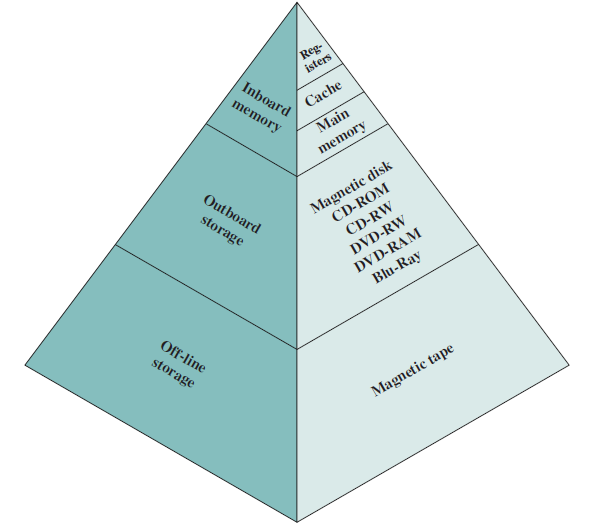
\includegraphics[width=.6\textwidth]{images/3_basics/mem-hierarch.png}
    \caption{Memory hierarchy\\Source: \cite[p. 125]{computerarch}}
    \label{fig:memhierarch}

\end{figure}


\begin{table}[H]
    \centering
    \renewcommand\tabularxcolumn[1]{m{#1}}
    \begin{tabularx}{\textwidth}{XXXXX}
    \hline
        \textbf{Level} & \textbf{1} & \textbf{2} & \textbf{3} & \textbf{4} \\ \hline
        Name & Registers & Cache & Main Memory & Disk Storage \\ \hline
        Typical Size & <4KiB & 32 KiB to 8 MiB  & <1 TB  & >1 TB \\ \hline
        Used\newline Technology & CMOS & CMOS SRAM & CMOS DRAM & Flash, Magnetic Disk \\ \hline
        Access time (ns) &  0.1–0.2  & 0.5–10  & 30–150  &  5,000,000 \\ \hline
        Frequency (MHz) & 10000-5000 & 2000-100 & 33-6 & 0.0002 \\ \hline
        Bandwidth (MiB/sec)  & 1,000,000–10,000,000  &  20,000–50,000  &  10,000–30,000  & 100–1000 \\ \hline
    \end{tabularx}
    \caption{Typical values for the different memory levels\\Source: \cite[p. 3]{quantivapproach-ApB}}
    \label{table:memhierarch}
\end{table}

The memory hierarchy design takes advantage of this principle by organizing data in different levels of the hierarchy based on their access patterns, with the faster and smaller memory closer to the processor and the slower and larger memory further away. This allows for faster and more efficient access to frequently accessed data, while less frequently accessed data can be stored in slower and larger memory. \cite[p. 127]{computerarch}

\section{Caches}

Level two memory in the memory hierarchy, or cache, is a small capacity memory which buffers a limited amount of recently accessed memory references. \cite[p. 94]{threeeasy} \cite[p. 23]{brendan}

When the processor loads a memory location, whether code or data, it first looks in the cache to see if it is already stored there. If it is in the cache, the processor fetches the information from the cache. This is called a cache hit. If the processor does not find it in the cache, the information has to be retrieved from main memory or the disk, which takes much longer than accessing the cache. This is called a cache miss. \cite[p. 2]{quantivapproach-ApB} \cite[p. 128]{computerarch}

% This is because the memory bandwidth increases as the numbers of cores grows.
Nowadays, the level two memory in the memory hierarchy no longer consists of a single cache but of a multilevel cache schema. The first-level cache can be designed to match the fast clock cycle time of modern processors, while the higher-level caches can be designed to have a larger capacity to store a significant amount of data from the main memory. This helps to reduce the number of times that the processor has to access the slower main memory. \cite[p. 78-83]{quantivapproach} 

The caches can be located either internally on the CPU die or externally. The exact depth, capacity and distribution of the caches depends on its type and model. \cite[p. 231-232]{brendan} An example can be seen in figure \ref{fig:cachehierarch}.

% In addition, logic density has increased over the years, allowing the cache to be on the same chip as the processor. Being on the same chip allows the cache to have its own bus with shorter data paths that are decoupled from the external bus. This reduces pressure on the external bus, which is shared with other components, and cache access time. \cite{computerarch} 

\vspace{.5cm}
\begin{figure}[H]
    \centering
    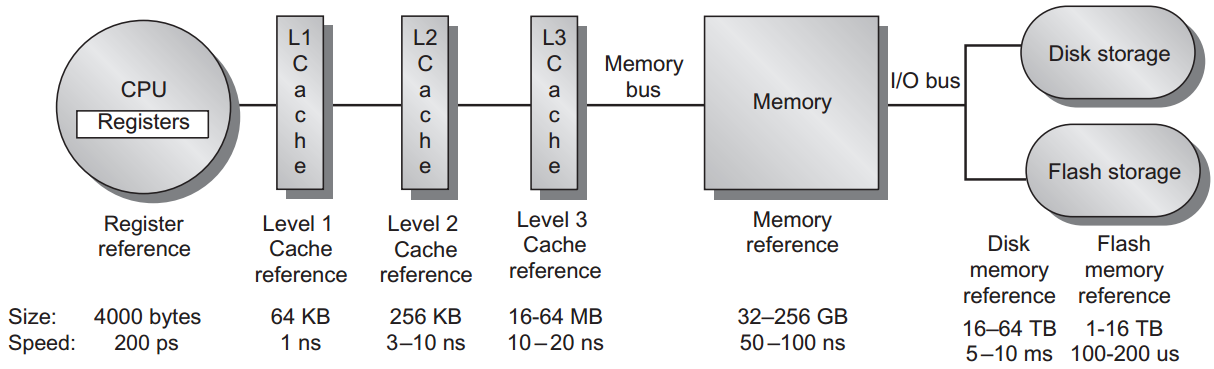
\includegraphics[width=\textwidth]{images/3_basics/caches.png}
    \caption{Memory hierarchy for an example server\\Source: \cite[p. 79]{quantivapproach}}
    \label{fig:cachehierarch}
    \vspace{-\baselineskip}
\end{figure}

Furthermore, individual caches can be split into separate instruction and data caches instead of a single unified cache. The trend is toward splitting the L1 cache into an instruction L1 cache (IL1 cache) and a data L1 cache (DL1 cache) and using a unified cache for higher levels. \cite[p. 149]{computerarch} 

The advantage of a split in the L1 cache is that it eliminates the contention between different units for a single cache in the pipeline. The disadvantage is that two caches have to be implemented instead of a single unified cache, which is more expensive. \cite{cache_memory} \cite[p. 147-149]{computerarch}

\section{Virtual Memory}\label{section:vm}

Virtual memory is an abstraction provided by the hardware to the processor. The operating system, which sets up and manages the virtual memory space for each process, enables the process to have its own virtual address space that maps to physical memory as needed. \cite[p. 133-134]{threeeasy} \cite[p. 194-195]{tanenbaum}

The addresses in this address space are so called \textit{virtual addresses}, which must be converted to the true \textit{physical memory address} before a memory access. This is called \textit{address translation}. It should be noted that this needs to be done for \textbf{all} processes and \textbf{every} memory access, in other words every time for example an instruction is loaded and executed in a program or the kernel. \cite[p. 133-134]{threeeasy} \cite[p. 195-196]{tanenbaum}

With this methodology, the kernel has the freedom to choose dynamically any memory place in physical memory for an address space which best suits the used memory layout scheme. \cite[p. 133]{threeeasy} \cite[p. 190-191]{tanenbaum}

Additionally, multiple virtual addresses in multiple processes can point to the same \textit{physical address}, such as for example in the case of shared libraries. Furthermore, the processes are protected from other processes, since the illusion prevails that they only run for themselves and use their own address space. \cite[p. 192, 137-138]{threeeasy} \cite[p. 228-230]{tanenbaum}

\section{Paging}\label{section:page}

Most virtual memory systems structure the memory in addition in the form of \textit{pages}. \textit{Pages} are chunks of memory of a program which are mapped to chunks of physical memory, called \textit{page frames}. \cite{virtual-memory} \cite[p. 195-196]{tanenbaum} The methodology of virtual memory in combination with paging can be seen in figure \ref{fig:singlepage} and \ref{fig:pagephysical}.

\begin{figure}[H]
     \centering
     \captionsetup{justification=raggedright}
     \begin{minipage}[b]{0.4\textwidth}
         \centering
         \hspace*{5mm}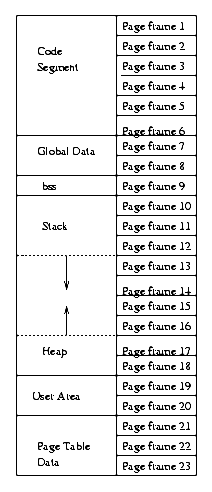
\includegraphics[height=8.5cm]{images/3_basics/pages-single.png}
         \caption{Address space of an example ELF file split in pages Source: \cite{pic:singlepage}}
         \label{fig:singlepage}
     \end{minipage}%
     \hspace*{7mm}
     \begin{minipage}[b]{0.6\textwidth}
         \centering
         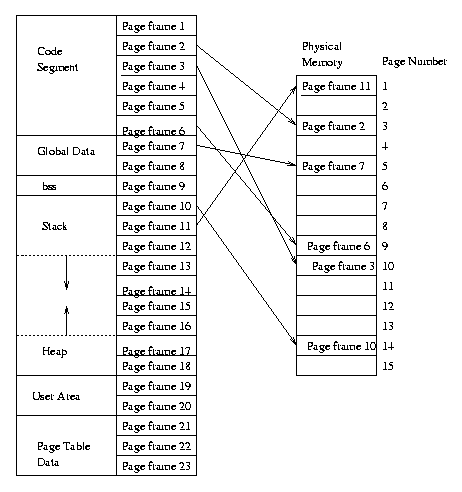
\includegraphics[width=.85\textwidth]{images/3_basics/pages-with-physical.png}
         \caption{Schematic representation of connections between virtual and physical pages\\
         Source: \cite{pic:singlephysical}}
         \label{fig:pagephysical}
     \end{minipage}
\end{figure}    
\vspace{-\baselineskip}

An advantage of this combination is that the kernel can load a physical address at a later point in time in order not to fill the physical memory prematurely and to leave free memory for other programs. This is called \textit{demand paging}. \cite[p. 240]{threeeasy} \cite[p. 299]{computerarch}

This information, which virtual page points to which physical page, is called a \textit{page table entry} (PTE). The kernel stores every PTE of every program combined in a \textit{page table}. In addition, a PTE stores more than the address translation. It also stores additional information like a valid bit, protection bits, \textit{present bit}, etc. \cite[p. 172-174]{threeeasy} \cite[p. 199-200]{tanenbaum}

The \textit{present bit} indicates whether the page has already been loaded into physical memory or not. If this has not happened at the time of the memory access, a \textit{page fault} is invoked and the page is loaded into physical memory from other storage, for example the hard drive.  \cite[p. 174]{threeeasy} \cite[p. 200]{tanenbaum}
\enlargethispage{\baselineskip}

Besides processing the address translation and other information bits in the PTE, the page table must first be looked through in order to find the entry for the virtual page. Searching the page table is also called \textit{page table walking}. \cite[p. 187]{threeeasy} \cite[p. 204-205]{tanenbaum}

\newpage

Instead of a simple linear page table, which is a simple list structure of all the PTEs, nowadays \textit{multi-level page tables} are used to reduce the size of the page table to be stored per process. This is also called a \textit{page directory}. However, this has the disadvantage that a multi-level page table is more complex to keep track of and look through when searching for a PTE than a linear page table. \cite[p. 205-207]{threeeasy} \cite[p. 205-207]{tanenbaum}

In order to relieve the processor of all this additional work, an extra hardware unit was designed that is dedicated to this task: the \textit{Memory Management Unit} (MMU). \cite[p. 135]{threeeasy} \cite[p. 195-196]{tanenbaum}\\
Figure \ref{fig:simplemmu} shows the positioning of the MMU in comparison to other components.

\begin{figure}[H]
    \centering
    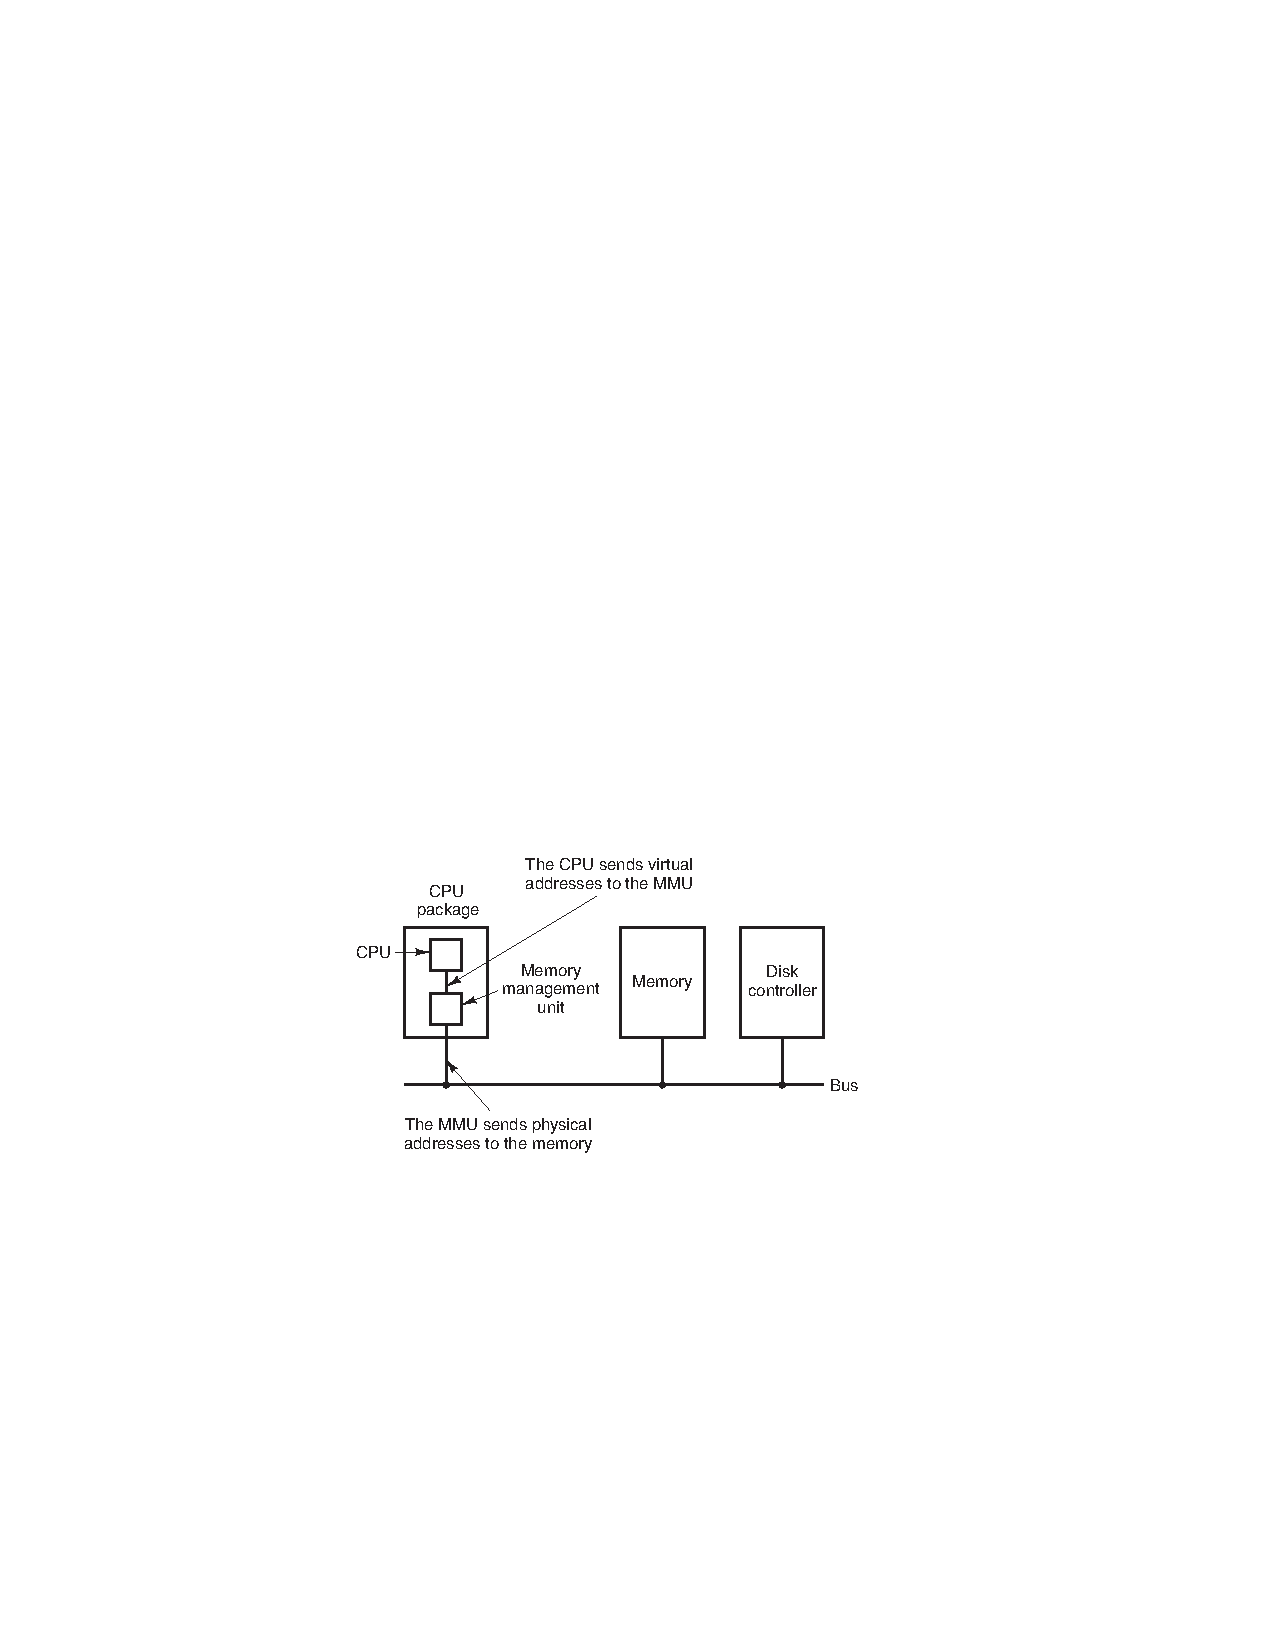
\includegraphics[width=.65\textwidth]{images/3_basics/hardware-paging.pdf}
    \caption{Hardware positions and connections\\Source: \cite{tanenbaum}}
    \label{fig:simplemmu}
\end{figure}
\vspace{-\baselineskip}

\section{Translation Lookaside Buffer (TLB)}\label{section:tlb}

To further speed up the address translation, a hardware cache was introduced that temporarily stores frequently accessed PTEs for use in the near future. This cache is located in the MMU itself and is called \textit{translation lookaside buffer}, or \textit{TLB} for short. It is a small cache which stores only a small amount of entries. \cite[p. 183]{threeeasy} \cite[p. 202]{tanenbaum}

When a memory access takes place, the MMU checks first the TLB to see if the desired PTE already exists in the TLB. If this is the case, a so called \textit{TLB hit}, the desired PTE is returned to the process. \cite[p. 184]{threeeasy} \cite[p. 203]{tanenbaum}

If this is not the case, the MMU starts the process of page table walking and, in the worst case, page faulting. This case is called a \textit{TLB miss}.  \cite[p. 184]{threeeasy} \cite[p. 204]{tanenbaum} If this happens multiple times because, for example, the cache full is or the wrong PTEs were stored, then one speaks of \textit{TLB pressure}.

Since the entries in the TLB are cached for the most frequently accessed PTEs per process, it is important to be careful that a process is not misinterpreting the remaining entries in the TLB by another process if a process switch happens. The simplest way to avoid this problem is to flush the entire TLB when a process changes, which is called \textit{TLB flush}. \cite[p. 191-192]{threeeasy} \cite{lwn_vm} \cite[p. 233-234]{tanenbaum} The entire process is illustrated in figure \ref{fig:memstatemachine} and \ref{fig:memaccesstime}.

\begin{figure}[H]
    \centering
    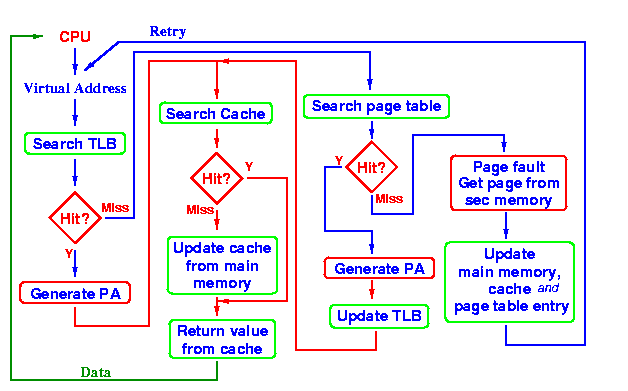
\includegraphics[width=.8\textwidth]{images/3_basics/mem_op.png}
    \caption{Flowchart of a memory access\\Source: \cite{pic:memop}}
    \label{fig:memstatemachine}
\end{figure}
\vspace{-\baselineskip}

Additionally, figure \ref{fig:memaccesstime} shows a more broken down example with additional approximate time sequences. From this schematic one can see that in the process of memory access through the MMU, page faults should be avoided as much as possible, because this leads to additional waiting times, especially if they occur frequently.

In modern systems, to profit from the principle of locality, the TLB is split in \textit{Instruction Translation Lookaside Buffer} (ITLB) and \textit{Data Translation Lookaside Buffer} (DTLB). \cite[p. 2, 4-5]{quantivapproach-ApL}

\vspace{\baselineskip}
\begin{figure}[H]
    \centering
    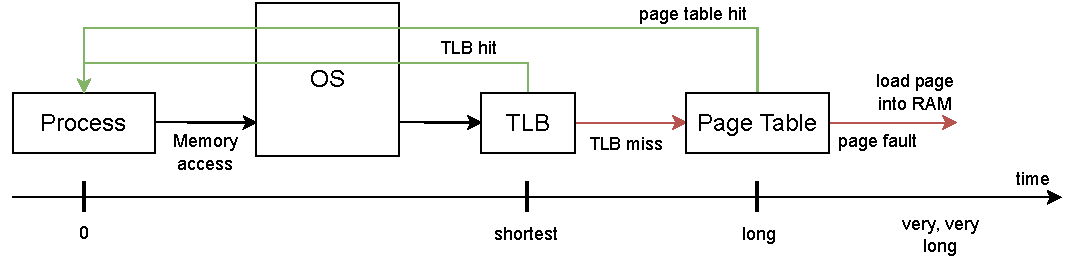
\includegraphics[width=\textwidth]{images/3_basics/mmu-more.pdf}
    \caption{Simple schematic of a memory access with time axis}
    \label{fig:memaccesstime}
\end{figure}
\vspace{-\baselineskip}

ITLB and DTLB are separated because instructions and data have different access patterns. Instructions are typically read sequentially, with the next instruction being located at a memory address that is close to the current instruction. On the other hand, data access patterns can be more random, with data being accessed from various locations and with random size in memory. \cite[p. 4-5]{quantivapproach-ApL}

\section{Performance Monitoring Unit (PMU)}\label{section:pmu}

The \textit{Performance Monitor Unit} (PMU) is a hardware component in modern computer processors that is used to measure various performance-related metrics such as the number of retired instructions executed, the number of cache misses, the number of branch mispredictions, etc. \cite[p. 156]{brendan} \cite{pmushort}

The PMU can be accessed by software through a set of registers which are used to configure the counters, read their values and calculate specific performance metrics like \textit{instructions per cycle} (IPC). \cite{how-counters-work} \cite[p. 681]{brendan} \cite{pmushort}

Depending on the processor model other features could be included like \textit{Last Branch Recording} (LBR), \textit{Event-Based Sampling} (EBS), \textit{Precise Event-Based Sampling} (PEBS) and other. \cite[p. 43]{patmc} The Linux kernel uses its own frontend tool \textit{perf}, which is an easy to use interface to access and configure the counters of the PMU. \cite[p. 671]{brendan}
\chapter{Conceptual analysis}\label{chapt:consider}

This chapter covers the discussion and analysis regarding the expected issues occurring during the upcoming design stage. The focus will be on two questions: how to \textit{analyze a program for a weighted call graph} and how to \textit{sort a weighted call graph into a linear layout}.

\section{Call graph analysis}\label{chapt:callgraph}

Call graphs show the relationship between call sites and functions, i.e. which caller function calls which other callee functions and vice versa. \cite[p. 133]{binanal} 

The number of calls where the caller invokes the callee can be counted during the runtime of the program. By dividing this value with the total amount of counted samples, a weight can be assigned to this relationship which describes how often the caller invokes the callee or vice versa during the runtime.

From this information a weighted call graph, or \textit{directed network}, can be created. \cite{graphintro} This can be done in two ways: with a \textit{static analysis} or a \textit{dynamic analysis}.

\subsection{Static analysis}

Static analysis is the process of analysing a program without executing it. It treats the program as data, which is then the subject for analysis. This can be done by examining the source code or the machine code of the program, as well as the data and metadata associated with it. \cite{binanal} \cite{lca-gcc-plugin} \cite{staticanalyze}

The advantage is that the program does not have to be executed, thus the result of the analysis is independent of a hardware unit. Additionally, the results of a static analyser are consistent: in comparison to an execution of the program on real hardware no external conditions such as temperature of the measuring room, noise interference or other interference sources can influence the result. \cite[p. 68]{patmc} \cite{staticanalyze}

The downside is that building a cost-effective program analyser is not easy, since most programs are complex and have many lines of code. This problem is further aggravated by the fact that for such programs there are countless combinations of inputs and countless program states which can be generated from them, to which the analyser must provide a deterministic result. \cite[p. 19]{staticanalyze}

Another challenge with static analysis is that an ideal static analyser would be able to fully analyse the desired property automatically within a finite amount of time. For instance, one such property could be determining whether a program is error-free during runtime. However, as demonstrated by the \textit{Halting Problem}, this is an unsolvable problem. \cite[p. 19]{staticanalyze}

The halting problem describes the limitation to identify whether a given program will halt or continue to execute indefinitely. It is proven that this property of interest is unsolvable. \cite[p. 23]{staticanalyze} This means that it can not be predicted beforehand if a program, for all possible inputs, finishes its execution.

In general, one can say that for any non-trivial property of a program, it is undecidable whether a given program has this property or not. This theorem is called \textit{Rice's Theorem}. \cite[p. 24]{staticanalyze}

This means that for any non-trivial property, that can't be decided by examining the program's inputs, there will always be a program for which it is impossible to determine whether that property applies or not. An example could be the property of a program being able to determine whether a given randomly selected program will output a prime number or not. Given an arbitrary program, it is not possible to determine whether this is the case or not.

The halting problem and Rice's theorem point to the fact that the output of a static analyser is not necessarily a deterministic result. This is because the used heuristics and approximations to relax the requirements for an ideal static analyser may not always work as intended, especially for more complex and optimized programs. \cite[p. 24-25]{staticanalyze}

It follows that a static analyser may produce false positives and false negatives, meaning that it may identify certain features or properties of a program that do not actually exist or misinterpret certain code wrongly. \cite[p. 25]{staticanalyze} Furthermore, some programs, e.g. malware, may use obfuscation or code packing techniques that make analysing them more difficult. In these cases, static analysis may need to be performed completely manually. \cite[p. 30]{staticanalyze} \cite[p. 13]{malware}

This thesis deals with the Linux kernel, which is a large and complex program. Therefore, it can be assumed that the above theorems and associated problems are applicable here. The resulting call graph could therefore represent incorrect relationships and weights.

Furthermore, the kernel is mainly written in \textit{C} programming language. Its low-level nature makes it possible to use complex pointer arithmetic, which complicates the creation of call graphs when e.g. indirect function calls are used. Additionally, the code following the preprocessor stage and the resulting compiled binary can differ greatly from each other depending on the architecture and entries selected for compilation. 

Moreover, the frequency and timing of system calls being invoked depends entirely on the user-space application in use and its specific implementation. Therefore, in order to obtain a realistic weighted call graph, it is necessary to not only statically analyse the kernel itself but also the application being employed, which increases the effort involved.

\vspace{-\baselineskip}
\subsection{Dynamic analysis}

In comparison to static analysis, dynamic analysis is the process of analysing the properties of a program while executing it on the hardware. \cite[p. 2]{binanal} It enables the identification of issues that may not be readily detected by static analysis. By collecting real-time information during the runtime, dynamic analysis can effectively capture and analyse the precise state of the program at any given moment. This allows for the detection of performance-related issues and other runtime-specific problems that static analysis may overlook. \cite{concept-dynamic}

\enlargethispage{3\baselineskip}
One downside of dynamic analysis that must be considered is the risk of measurement bias. Measurement bias is the tendency for measurements to be inaccurate due to errors or imprecision in the measurement process. However, completely eliminating it can be challenging because it is unpredictable when and where it may occur. \cite[p. 17-19]{patmc} \cite{wrong-data}

In addition, the impact of noise, external side effects and similar sources of interference during the analysis must be minimized as much as possible as not to distort the result. \cite[p. 69]{patmc}

\newpage

On top of that, the observer effect has to be taken into account. The observer effect states that measuring a property affects the observation because running the observer itself uses CPU cycles in order to observe the running program. This has the consequence that the analyser can influence e.g. how caching is done, how memory is allocated, etc. \cite[p. 20]{patmc} \cite[p. 387]{masterembedded} Therefore, it is important that the dynamic analyser has as little overhead as possible, i.e. uses as few CPU cycles as possible for its observation task. 

Various techniques, including instrumentation, tracing, and sampling, can be employed to observe and analyse the performance of a running program. \cite[p. 52]{patmc}

Instrumentation and tracing insert additional code to collect information during the runtime. To do this, the code must be modifiable. In comparison, tracing focuses on monitoring the interactions between a program and its external dependencies, such as libraries or other services, which may already have some form of instrumentation. Therefore, the program itself does not have to be modified. \cite[p. 52-55]{patmc}

Compared to instrumentation and tracing, sampling, also called \textit{profiling}, interrupts the running program to capture a new sample. This sample is a snapshot of the current program state, which can be e.g. the value of the instruction pointer at the time of the interrupt. Sampling provides a coarse view of the targets activity, depending on the sampling frequency. \cite[p. 35]{brendan} \cite[p. 59]{patmc}

Instrumentation and tracing offer the advantage of generating precise and detailed data of the program state. However, they can introduce significant overhead and generate large amounts of data, depending on the type and amount of information collected. Additionally, a version of the program with and without instrumentation or tracing enabled must be compiled to avoid additional runtime overhead during e.g. performance tests. \cite[p. 53-54]{patmc} \cite{bolt}

In comparison, sampling does not produce as precise data as instrumentation or tracing, but has a much lower overhead during runtime. The precision of the data collected through sampling can be improved by increasing the number of samples. \cite{hfsort} \cite{bolt} The kernel has its own infrastructure for instrumentation as well as sampling.

\enlargethispage{3\baselineskip}
Because of an additional build for data collection and a very significant CPU and memory overhead, instrumented binaries are not used in production environments. \cite{bolt} Nonetheless, these techniques are employed in other tools like e.g. \textit{Propeller} \cite{propeller}.

\section{Function-ordering heuristics}\label{chapt:heuristic}

\textit{Function-ordering} or \textit{function placement} is a subset of \textit{feedback-driven optimizations} (FDO) or also called \textit{profile-guided optimizations} (PGO). \cite[p. 122]{brendan} \cite{bolt}

PGO aims to enhance the performance of a program by collecting information about its actual runtime behaviour, such as function call frequencies and hot code paths, and uses that information to guide optimization decisions during compiling. \cite{kernel_pgo} \cite[p. 122]{brendan} \cite{intelpgo}  This covers a large area of optimisation techniques such as \textit{basic block placement}, \textit{basic block alignment}, \textit{function splitting} and more. Explanations and examples for these can be found in \cite[p. 103-111]{patmc}. This thesis however focuses only on the effects of using a function sorting heuristic. 

Heuristics are employed because, if $P \neq NP$, function-ordering is an NP-hard problem, i.e. this problem can't be solved in polynomial time. \cite{codestitcher}  \cite{np-hard-explained} \cite{nphard} The most common function-sorting heuristic implemented in compilers, binary optimizers and performance tools is the \textit{procedure ordering} heuristic, which is described in \cite{phheuristic}. It is also referred to as \textit{Pettis-Hansen} (PH) heuristic. \cite{codestitcher} \cite{hfsort}

The PH heuristic is based on an \textit{undirected} weighted call graph, where the distinction between caller and callee functions is not considered, but the weight between them is known. It processes this graph in decreasing weight order, merges the two functions associated with their weight together and adds their total weight up. It proceeds until all weights are analysed. \cite{anticodestitcher} \cite{hfsort}  \cite{phheuristic}

Building upon the PH heuristic is the \textit{Call-Chain Clustering} (C3) heuristic, described in \cite{hfsort}. C3 differs from the PH heuristic in several ways: it utilizes a directed call graph that incorporates the total call-distance and sorts the merged functions based on a density metric.

Based on the findings presented in \cite{hfsort}, the C3 heuristic demonstrates an average reduction of ITLB misses by approximately 12\% compared to the PH heuristic. The evaluation further concludes that through the use of the C3 heuristic the analyzed application experiences a performance gain of up to 2.9\% when compared to the PH heuristic. At the time of writing the C3 heuristic is used in the \textit{BOLT} project \cite{bolt} which got integrated into the LLVM project. \cite{bolt-in-llvm} There have also been attempts to integrate \textit{BOLT} into the kernel. \cite{bolt-kernel} 

\enlargethispage{2\baselineskip}
Although other techniques unrelated to function sorting, such as neural networks, could be applied, the author is not aware of any papers that have specifically explored their use for function ordering at this time.
\chapter{Implementation}\label{chapt:implement}

This chapter describes the implementation of the chosen test procedure and the related test parameter. Afterward, the results are presented and interpreted. The test procedure consists of the following stages:

% start item counter at zero
\begin{enumerate}\addtocounter{enumi}{-1}
    \itemsep-1.3em 
    \item Describe the workloads and parameters by which a system is to be tested.
    \item Test the unoptimized system using the specified workloads and parameters.
    \item Generate a weighted call graph from the workload on the unoptimised system.
    \item Sort the weighted call graph into a linear list using a function-ordering heuristic.
    \item Create a new optimised system using this linear list.
    \item Test the optimised system using the specified workloads and parameters.
\end{enumerate}

An Intel Core i3-6100U CPU with skylake microarchitecture is used as the test processor. This model features a 4KiB ITLB and DTLB with 64 entries and a shared 4KiB second level TLB with 1536 entries. Furthermore, each core has its own L1 data cache, L1 instruction cache and L2 cache. The L3 cache is shared between all cores. \cite{cpuinfo} 

The implementation is based on the performance analyse tool \textit{perf}, which is readily available in the kernel. The complete implementation can be found at \cite{github}, while simplified code snippets can be found in chapter \ref{appendix:implement}.

\vspace{-\baselineskip}

\section{Workload}

\enlargethispage{2\baselineskip}
For the implementation of the workloads, it is important that these predominantly affect functionality in the kernel space, i.e. they need to be kernel centric. This means that rather than CPU intensive workloads which run mostly in user space, there will be workloads that focus on stressing kernel tasks like network, scheduler, filesystem, etc.

That said, the objective is not to optimise the whole kernel but rather subsystems of it because there is functionality in the kernel where optimization is not useful for the performance, such as for example the \textit{debugfs} filesystem.

In order to avoid possible causes of interference, it is advisable to interact as little as possible with external components. For example, in workloads like databases which involve heavy disk I/O operations, the workload will be I/O-bound. This means the measurement will include the time taken for data transfers between the disk and the system, thus diverting the focus away from kernel centric tasks.

Furthermore, to create a more realistic workload scenario, it was decided to run the workload on a Linux operating system with a desktop environment. At the time of writing, the latest stable version of Debian bullseye was used as the base. This approach helps to create a more accurate end result, as it mimics a more real world environment for the workload, thus providing a clearer recommendation for the use of code collocation in the kernel for an end user. The disadvantage of this, however, is that other causes and effects of interference can creep in and blur the results of the analysis.

For this thesis a network driven workload was chosen. An attempt was made to implement a database workload, but it did not demonstrate the same degree of precise repeatability as a network workload. Furthermore, it is important to ensure that the workload is sufficiently intense during runtime to overshadow other processes running in user space which could also access the kernel space at the runtime of the workload. This can be achieved with an increased workload priority and an increased number of workload processes.

Furthermore, one could fine-tune parameters for the network workload in order to achieve a more frequent traversal of the network code in kernel space. For example, the \textit{direct memory access (DMA) ring buffer} could be set to the minimum for the used network card.

\enlargethispage{3\baselineskip}
This fine-tuning option is used in this thesis for the call stack analysis, but not for the analysis of the PMU events. The reason is that in the call stack analysis, it is important to create as precise a weighted call graph as possible. The higher precision result, which is acquired from the frequent traversal of the code, then affects the function-sorting heuristic as well as the final linear list. However, for the actual workload test where the PMU events are analysed, it is important to expose them to more real-world circumstances. Since most people do not change these parameters but use the default values, there could be a risk of blurring the final result of the analysis.

\section{PMU events}\label{section:events}

The selection of the PMU events strongly determine the interpretation of the results and must therefore be carefully chosen. As different processor models may have different PMU events implemented, it is important to select those that provide a more concrete interpretation of the objective.

% In addition, one should note that ITLB misses are caused by an instruction fetch, which happen primarily in the frontend of the pipeline.
In this thesis, the aim is to reduce ITLB pressure, so PMU events were chosen to measure the number of ITLB misses, CPU stalls, or page table walks during the runtime of the workload. The following PMU events from \cite{skylake_events}, with the help of  \cite[p. 266]{brendan} and \cite{propeller}, were chosen for the used processor model:

\begin{itemize}
    \item \spcstring{ITLB_MISSES.MISS_CAUSES_A_WALK}\\
    "Counts page walks of any page size (4K/2M/4M/1G) caused by a code fetch. This implies it missed in the ITLB and further levels of TLB, but the walk need not have completed." \cite{skylake_events}
    \item \spcstring{ITLB_MISSES.WALK_ACTIVE}\\
    "Cycles when at least one [Page Miss Handler] is busy with a page walk for code (instruction fetch) request. [Extended Page Table] page walk duration are excluded in Skylake microarchitecture." \cite{skylake_events}
    \item \spcstring{ITLB_MISSES.WALK_COMPLETED}\\
    "Counts completed page walks (all page sizes) caused by a code fetch. This implies it missed in the ITLB (Instruction TLB) and further levels of TLB. The page walk can end with or without a fault." \cite{skylake_events}
    \item \spcstring{FRONTEND_RETIRED.ITLB_MISS}\\
    "Counts retired Instructions that experienced iTLB (Instruction TLB) true miss." \cite{skylake_events}
    \item \spcstring{ICACHE_64B.IFTAG_MISS}\\
    "Instruction fetch tag lookups that miss in the instruction cache (L1I). Counts at 64-byte cache-line granularity." \cite{skylake_events}
\end{itemize}

The distinction between retired instructions and code or instruction fetch must be taken into consideration. The PMU events described here could also count code or instruction fetches that were loaded and executed via speculative execution. \cite[p. 34-35, 46]{patmc} \cite{intel_retired}
\enlargethispage{\baselineskip}

This means that if an instruction loaded by the speculative execution is not needed, because for example the prediction was wrong, this instruction will be not retired and consequently flushed, i.e. the instruction will be not written back. Retired instructions are therefore instructions which are correctly predicted and successfully written back. \cite[p. 46]{patmc} \cite{intel_retired}

Intel has published a white paper on the subject of reducing ITLB miss stalls, which can be found at \cite{intel_opt_runtime}. They define metrics which can be also used in this thesis:

\begin{itemize}
    \item ITLB Stall Metric\\
    "This metric represents the fraction of cycles the CPU was stalled due to instruction TLB misses." \cite{intel_opt_runtime}
    \begin{align*}
        ITLB\_Miss_{stall} = 100 \cdot 
        \left( \frac{\spcstring{ICACHE_64B.IFTAG_STALL}}{\spcstring{CPU_CLK_UNHALTED.THREAD}} \right)
    \end{align*}
    \item  ITLB Misses Per Kilo Instructions (MPKI)\\
    "This metric is a normalization of the ITLB misses against number of instructions, and it allows comparison between different systems." \cite{intel_opt_runtime}
    \begin{align*}
        ITLB\_MPKI = 1000 \cdot \left( \frac{\spcstring{ITLB_MISSES.WALK_COMPLETED}}{\spcstring{INST_RETIRED.ANY}} \right)
    \end{align*}
\end{itemize}

PMU events can be used in two modes: counting and sampling. Counting mode is used to count the total number of occurrences of specific events within a certain time period, while sampling mode saves the instruction pointer at the time of the occurrence of the event. \cite[p. 55-56, 59-60]{patmc} \cite[p. 157-158]{brendan} In this thesis, counting mode will be used to check for a significant change in the selected events. It is important to note that the total number of events counted in a certain time period may vary depending on the system's state.
\vspace{-\baselineskip}

\section{Call stack analysis}

% Honorable mentions:
% https://easyperf.net/blog/2019/02/09/Top-Down-performance-analysis-methodology
% https://easyperf.net/blog/2019/08/02/Perf-measurement-environment-on-Linux#8-use-statistical-methods-to-process-measurements
% https://www.intel.com/content/www/us/en/docs/vtune-profiler/cookbook/2023-1/top-down-microarchitecture-analysis-method.html
% https://github.com/intel/perfmon

The chapter \ref{chapt:callgraph} serves as a basis for creating a weighted call graph for a specific workload. Although the creation of a weighted call graph can be done by static analysis, it is not recommended. Therefore, the weighted call graph will be analysed dynamically.

In order to obtain a realistic result, the overhead should be as minimal as possible, which is why profiling is used instead of tracing. To generate a call graph \textit{perf} supports the collection of call stacks, which captures the call stack at the time of the occurrence of the event. With the addition of a stack unwinder a call graph can be created out of the collected call stacks. \cite[p. 62]{patmc} \cite{stack-unwinder} 

A hardware feature which is recommended in several papers, projects and articles for the collection of call stacks is the \textit{last branch recording} (LBR) which further decreases the overhead of profiling. \cite{codestitcher, bolt, propeller, lwn-lbr} LBR uses model specific registers to store the last taken branches. \cite{easyperf-lbr} \cite{lwn-lbr} The LBR feature is in combination with \textit{perf} only supported for user call chains and not kernel call chains. \cite{man-perf-record}

The PMU event to be sampled on can be either \textit{cycles} or \textit{instructions}. However, \textit{cycles} is recommended because "empirically we found it to produce better results". \cite{llvm-bolt} It is also recommended by \cite{brendan-perf} to sample at an odd frequency of, for example 99Hz, instead of 100Hz to avoid locksteping. In addition, in this thesis the call graph will not be generated from profiling specifically the workload, but it will be generated from a system-wide profiling of the kernel space for each CPU. This has the advantage of capturing the entire system's execution, including interactions between different processes and threads. 

To further enhance the creation of call graphs, the used processor has a built-in  hardware feature called \textit{hardware event-based sampling} (EBS) and \textit{processor or precise event-based sampling} (PEBS). \cite[p. 158]{brendan}

EBS does not interrupt the process each time the event occurs, but only when the associated counter overflows, at which point the instruction pointer is collected. \cite[p. 59-60]{patmc} \cite{brendan-perf} The advantage of not collecting a sample for each interrupt but waiting for an overflow is the reduction in overhead and collected data size. Since it is not of interest which instruction pointer is present for every CPU cycle, the total number of information and the number of saved and to be evaluated samples can be reduced. With a large enough sample size, if the program is executed long enough, the results are as statistically important as without EBS. \cite[p. 59-60]{patmc} \cite{brendan-perf} \cite{intel_ebs}

Nevertheless, there is a risk of a possible delay between the event overflow and the collection of the instruction pointer with EBS, which results in recording an incorrect instruction pointer at the time of the overflow. The result is a wrong recording of the code line which has caused the overflow. This inaccuracy is called \textit{skid}. A hardware feature which the used processor implements to combat skid is PEBS. \cite[p. 158]{brendan} \cite{intel_skid}
\enlargethispage{\baselineskip}

Both the \textit{BOLT} project \cite{llvm-bolt} and the \textit{Propeller} project \cite{llvm-propeller} use the EBS functionality, but without PEBS. Whether the usage of the PEBS functionality will create a more precise weighted call graph is not known.

\section{Function ordering and compilation}

In order to evaluate the collected call stacks and create a linear list for the compilation, the raw data must be first converted into usable information for the function-sorting heuristic, i.e. into a weighted call graph. An example weighted call graph can be seen in figure \ref{fig:excallgraph}.

\begin{figure}[H]
    \centering
    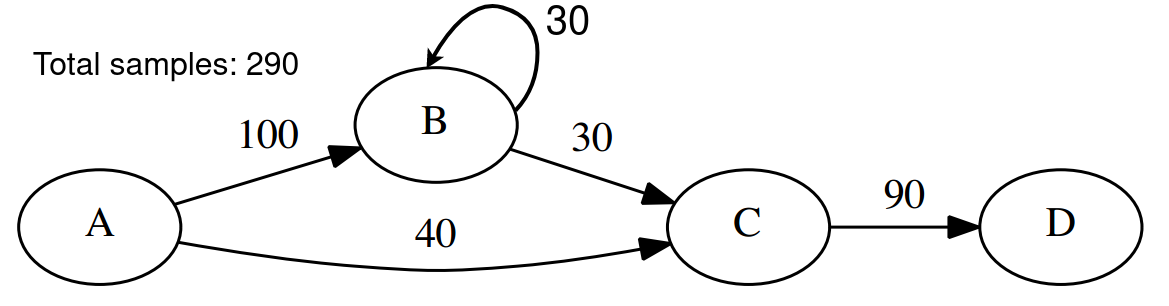
\includegraphics[width=.7\textwidth]{images/5_implementation/c3-custom-example.png}
    \caption{Modified example of a weighted call graph\\Source: \cite{hfsort}}
    \label{fig:excallgraph}
    \vspace{-\baselineskip}
\end{figure}

The parameters which are needed for the function-sorting heuristic can be acquired via an included raw data parser implementation of \textit{perf}. With this, important parameters such as unique caller-callee calls and the number of calls during the duration of the running system can be determined from the collected call stacks. Although \textit{perf} provides its own implementation interface for direct access to the raw data, this thesis has chosen to use the included implementation to obtain the necessary information.

Unfortunately, the included implementation of \textit{perf} creates cyclic node information, i.e. information which describes that a node calls itself. In the figure \ref{fig:excallgraph} an example can be seen where the node \textit{B} calls itself.  These samples can occur through, for example, recursive functions. This thesis considers cyclic nodes as part of the weighted call graph and includes them in the function-sorting heuristic accordingly. Any symbol names, i.e. function names, that were not obtained from the collected function pointers are sorted out.

\newpage

The function-sorting heuristic used in this thesis is the C3 heuristic because it offers better performance results than the PH heuristic. To implement the C3 heuristic, a weighted call graph and the function size of each individual function are required. This information can be obtained with \textit{perf}. The function size can alternatively be obtained via the generated \textit{System.map} file during the kernel compilation or via the \textit{kallsyms} functionality of the executed kernel.

For the C3 heuristic, it is also assumed that the total time spent in a node is equal to the sum of the incoming arcs. Accordingly, a cyclic node is included in the calculation of the total time of a node or the density of the individual clusters. A page size of 4KiB is specified, although other page sizes are possible.

The original authors have already implemented the C3 heuristic in the \textit{hfsort} utility, which is part of the \textit{hhvm} project \cite{hhvm}. This implementation generates a linear list from the weighted call graph, which can be used in the linker phase of compilation. To move individual sections, i.e. individual functions, in the linker phase, the kernel must be compiled with the compilation flag \textit{-ffunction-sections}.
\section{Evaluation and Results}\label{chapt:results}

The results shown here were executed with the previously mentioned settings. The two labels \textit{optimized} and \textit{unoptimized} refer to the two different compiled kernels. The label \textit{unoptimized} means a kernel which was compiled with the default settings, the label \textit{optimized} means a kernel compiled with the custom sorted linker script. Both kernels are of version \textit{5.10.178} and were compiled with \textit{gcc-10}. The flag \textit{nokaslr} was used as an additional boot parameter.

A group of network applications was selected on which both the call stack analysis and the PMU events collection were performed. Each kernel was tested five times. PMU events were counted for 6 hours with a sampling period of 1 second, resulting in 21,600 samples per test run. Call stacks were collected for 140 seconds to avoid losing any information. A warm-up time of 10 minutes was used for each collection. Recommended settings and parameters are included from the BOLT project \cite{llvm-bolt}. Table \ref{table:numberresults} presents the geometric mean of the collected PMU events for both the optimized and unoptimized cases across all test runs.

\begin{table}[H]
    \centering
    \begin{tabular}{clccc}
        &&&&\\ [-3mm] \hline
        & \multicolumn{1}{c}{\multirow{2}{*}{PMU events and metrics}}   & \multicolumn{2}{c}{Counted values for case} & Difference \\ \cline{3-4}
        && \multicolumn{1}{c}{unoptimized} & \multicolumn{1}{c}{optimized} & in percentage  \\ \hline
        &&&&\\ [-4mm]
        \triadown & itlb\_misses.miss\_causes\_a\_walk & 1584215 & 1571755 & -0.787 \\
        \triadown & (kilo) itlb\_misses.walk\_active & 71240 & 70675 & -0.793 \\
        \triadown & itlb\_misses.walk\_completed & 726417 & 713469 & -1.782    \\
        \triadown & frontend\_retired.itlb\_miss & 359667 & 143449 & -60.116 \\
        \triadown & icache\_64b.iftag\_miss & 148360051 & 136604656 & -7.924   \\
        &&&&\\ [-3mm]
        \triaup & IPC & 2.5775 & 2.6011 & 0.916 \\
        \triadown & ITLB Stall & 2.5815 & 2.4337 & -5.725  \\
        \triadown & ITLB MPKI & 0.2036 & 0.2018 & -0.884  \\ 
        &&&&\\ [-4mm] \hline
    \end{tabular}
    \caption{Calculated geometric mean values for defined PMU events and metrics}
    \label{table:numberresults}
\end{table}
\vspace{-\baselineskip}

The first value in each row indicates whether the event or metric described should be minimized (\triadown) or maximized (\triaup). This is followed by the name of the PMU event or metric, which were defined in chapter \ref{section:events}, and the average counted value in the specified time period for the optimized and unoptimized kernel. The last column shows the calculated difference as percentage between the optimized and unoptimized values. A positive percentage indicates that the optimized value is larger than the unoptimized value, and vice versa. Additionally, the metric \textit{instructions per cycle} (IPC) has been included as reference for the general system performance.

However, the PMU events themselves are not a simple indicator of whether there is a measurable performance improvement for the application, such as faster compilation times or more searches per second. These values offer a more user-friendly way to evaluate the impact of code collocation on performance. Therefore, in addition to the PMU events, the average throughput for a network application, which is recommended for this type of application by \cite{intel_demistify}, was also tested. The throughput metric displays how much data can be sent or received during a time period. \cite[p. 22]{brendan} 

In this case, the network metrics \textit{throughput} and \textit{total bytes transferred} from the client to the server were measured for a single application on each kernel. The measurements were conducted five times, with each test run lasting for one hour. The zero-copy functionality was utilized during the measurements. In table \ref{table:throughput} displays the geometric mean of the collected measurements for both the optimized and unoptimized cases.

\begin{table}[H]
    \centering
    \begin{tabular}{clP{2cm}P{2cm}c}
        &&&&\\ [-3mm] \hline
        &\multicolumn{1}{c}{\multirow{2}{*}{Network metrics}} & \multicolumn{2}{c}{Counted values for case} & Difference \\ \cline{3-4}
        && \multicolumn{1}{c}{unoptimized} & \multicolumn{1}{c}{optimized} & in percentage  \\ \hline
        &&&&\\ [-4mm]
        \triaup & Throughput (kbit/s) & 20032754.27 & 22920552.65 & 14.415 \\
        \triaup & Total bytes (TB) & 8.198 & 9.375 & 14.357 \\
        &&&&\\ [-4mm] \hline
    \end{tabular}
    \caption{Calculated geometric mean values for throughput and total bytes transferred}
    \label{table:throughput}
\end{table}
\vspace{-\baselineskip}

Firstly, it is essential to exercise caution when interpreting the shown results, as they are specific to the test setup, the workload type and the conditions applied. Furthermore, it is important to highlight that these values have not undergone significance testing, and the results from other tests may exhibit significantly different outcomes.

In general, a positive trend can be observed in the events and metrics presented in table \ref{table:numberresults}. Although most of the events and metrics do not exhibit a significant impact from code collocation, there are three specific values that stand out: \textit{icache\_64b.iftag\_miss}, \textit{frontend\_retired.itlb\_miss}, and the \textit{ITLB Stall} metric, which exhibit reductions ranging from 5.725\% to 60.116\%. To further analyse these events and metric, their histogram distributions are to be examined.

Notably, only these two PMU events and this one metric have experienced a significant reduction impact from code collocation. This is likely due to the specific measurements performed by each event. The events, namely \textit{itlb\_misses.miss\_causes\_a\_walk}, \textit{itlb\_misses.walk\_active}, \\\textit{itlb\_misses.walk\_completed}, and along with the metric \textit{ITLB MPKI}, which incorporates the event \textit{itlb\_misses.walk\_completed}, count the amount, or cycles, of page table walks performed by executed instructions. 

This suggests that code collocation did not result in a reduction of not written back speculative executed instructions, as the workload continues to generate a similar number of page table walks even with code collocation. This situation can arise when, for instance, a cold page is to be fetched due to the branch predictor, but it is not present in the ITLB, prompting a page table walk. However, during the page table walk, it is recognized that the cold page is unnecessary, leading to the termination of the page table walk. Despite the page table walk being terminated, the page table walk caused by the fetching of the cold page is still classified as such and counted accordingly.

\newpage

In contrast icache\_64b.iftag\_miss, frontend\_retired.itlb\_miss, and the ITLB Stall metric, which incorporates the event \textit{icache\_64b.iftag\_stall}, are not as dependent on speculative execution as the other PMU events. Instead, they monitor stalls and misses that occur during instruction fetch tag lookup or count the number of retired ITLB instructions which did experience ITLB misses.

The histograms for the outstanding events can be seen in figure \ref{fig:histograms}. These histograms illustrate the events or metrics recorded per second and their frequency throughout all test runs. The data used in these histograms is based on the results from all five test runs, amounting to a total of 108000 samples per case. The mean value $\boldsymbol\mu$ and the standard deviation $\boldsymbol\sigma$ were calculated for each individual case.

The histograms provide validation for the results, as indicated in table \ref{table:numberresults}. All figures show a decrease in their values for the optimized case when compared to the unoptimized case, as illustrated in table \ref{table:numberresults}.

The presence of tails or other irregularities in the distributions, representing the influence of interfering sources, can be attributed to the test configuration. Despite prioritizing the network workload, the impact of other user space applications is still noticeable across all three figures. However, it is also evident that the adjustment of the priority of the workload had the desired effect, as a noticeable and measurable change can be observed. This influence does not appear to be as pronounced in the distribution in figure \ref{fig:histograms-stall} compared to the other distributions.

Of particular interest for interpretation is the distribution presented in figure \ref{fig:histograms-frontend} in combination with the geometric mean in table \ref{table:numberresults}. As this PMU event represents the count of retired instructions, the resulting data provides a more accurate and precise interpretation of ITLB pressure compared to PMU events which also include executed instructions, making it harder to assess the true impact of code collocation on ITLB pressure. In these test runs did not only the geometric mean decrease by approximately 60\%, but the standard deviation decreased also by around 65.86\%, from approximately 160381 to 54744.

\enlargethispage{\baselineskip}
The reduction in both the mean value and the standard deviation signifies a positive impact of code collocation. Firstly, the reduced mean value indicates fewer retired ITLB misses on average, which suggests an increase in ITLB hits. This, in turn, should lead to a decrease in ITLB stalls, as figure \ref{fig:histograms-stall} illustrates. Secondly, the reduced standard deviation implies less scattering and more consistent outcomes, indicating that the processor can rely more frequently on the pages stored in the ITLB for different operations, reducing in sum the need to fetch additional pages.

\newpage
\begin{figure}[H]
    \centering
    \begin{subfigure}{\linewidth}
        \centering
        \captionsetup{singlelinecheck=false, margin={28mm,0cm}}
        \caption{Event icache\_64b.iftag\_miss}
        \label{fig:histograms-miss}
        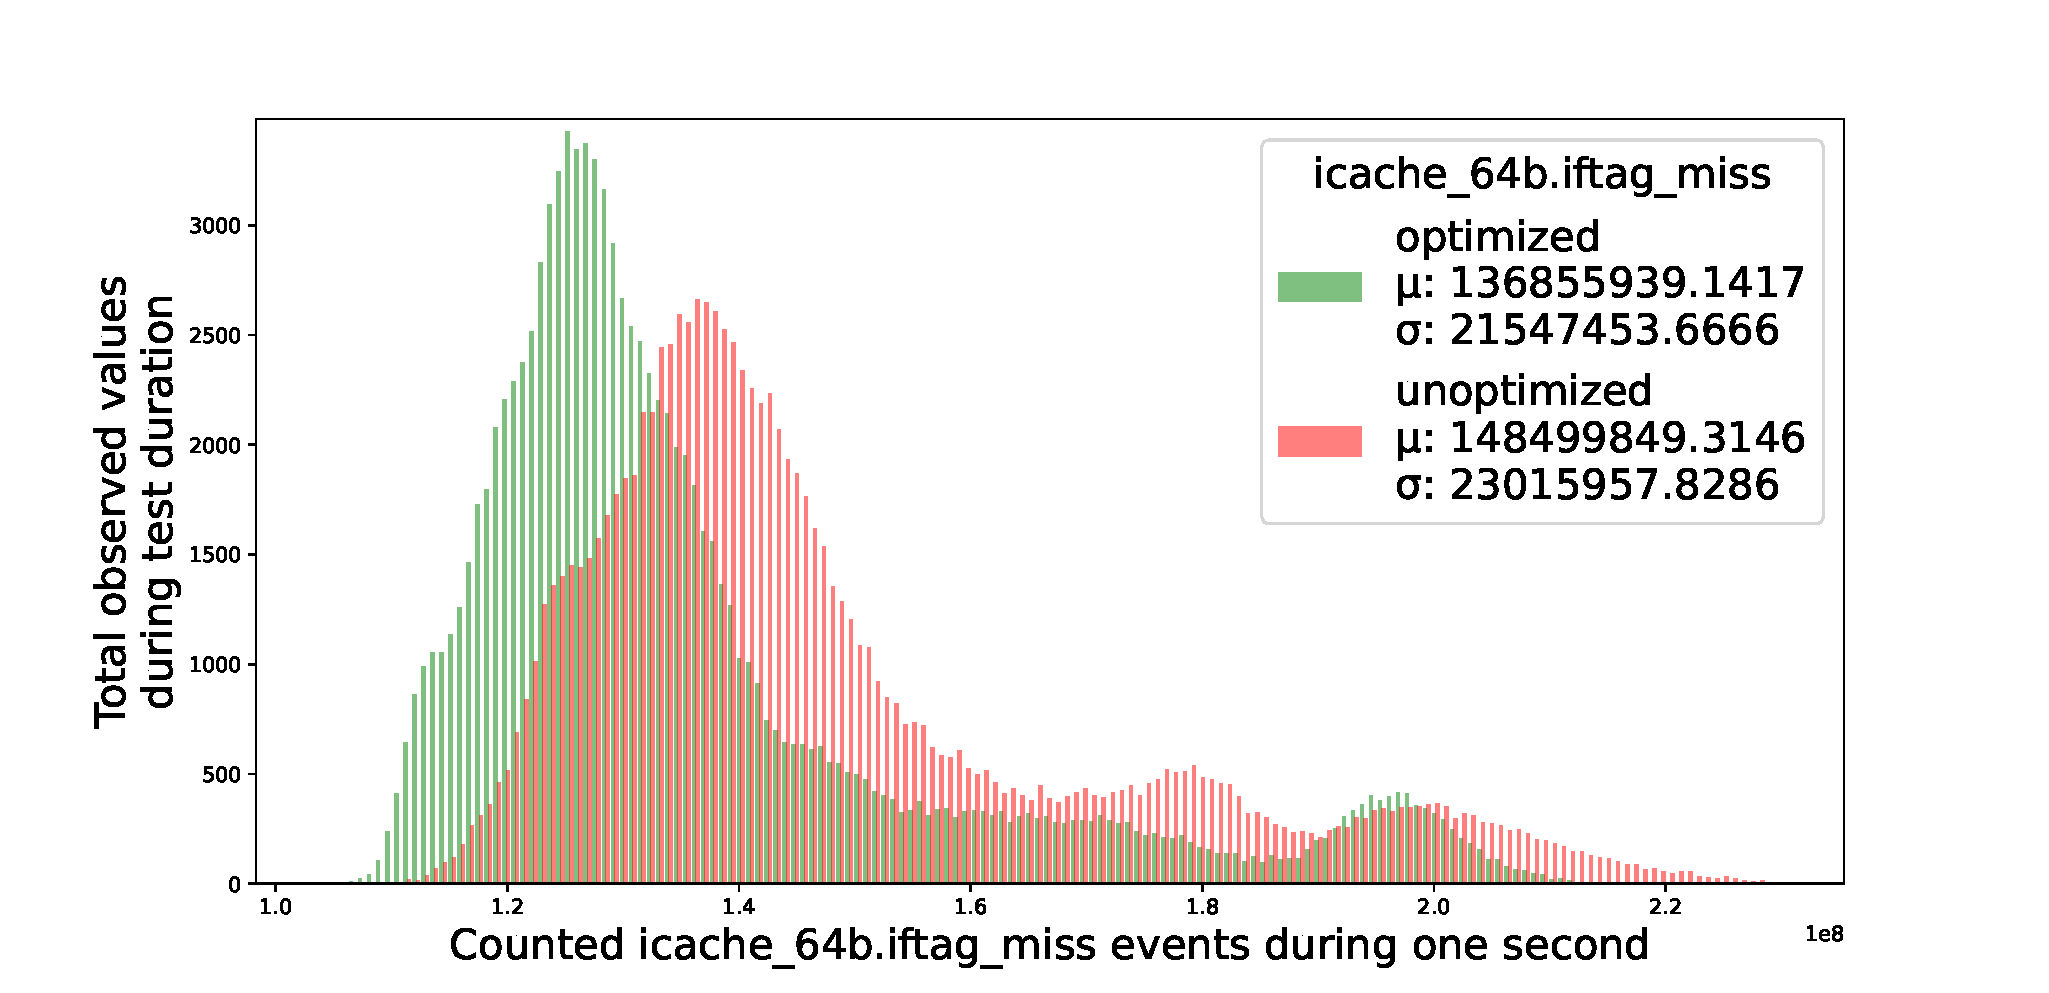
\includegraphics[width=.8\textwidth]{images/5_implementation/icache-iftag-miss.pdf}
        \vspace{.5\baselineskip}
    \end{subfigure}
    \begin{subfigure}{\linewidth}
        \centering
        \captionsetup{singlelinecheck=false, margin={29mm,0cm}}
        \caption{Metric ITLB stall}
        \label{fig:histograms-stall}
        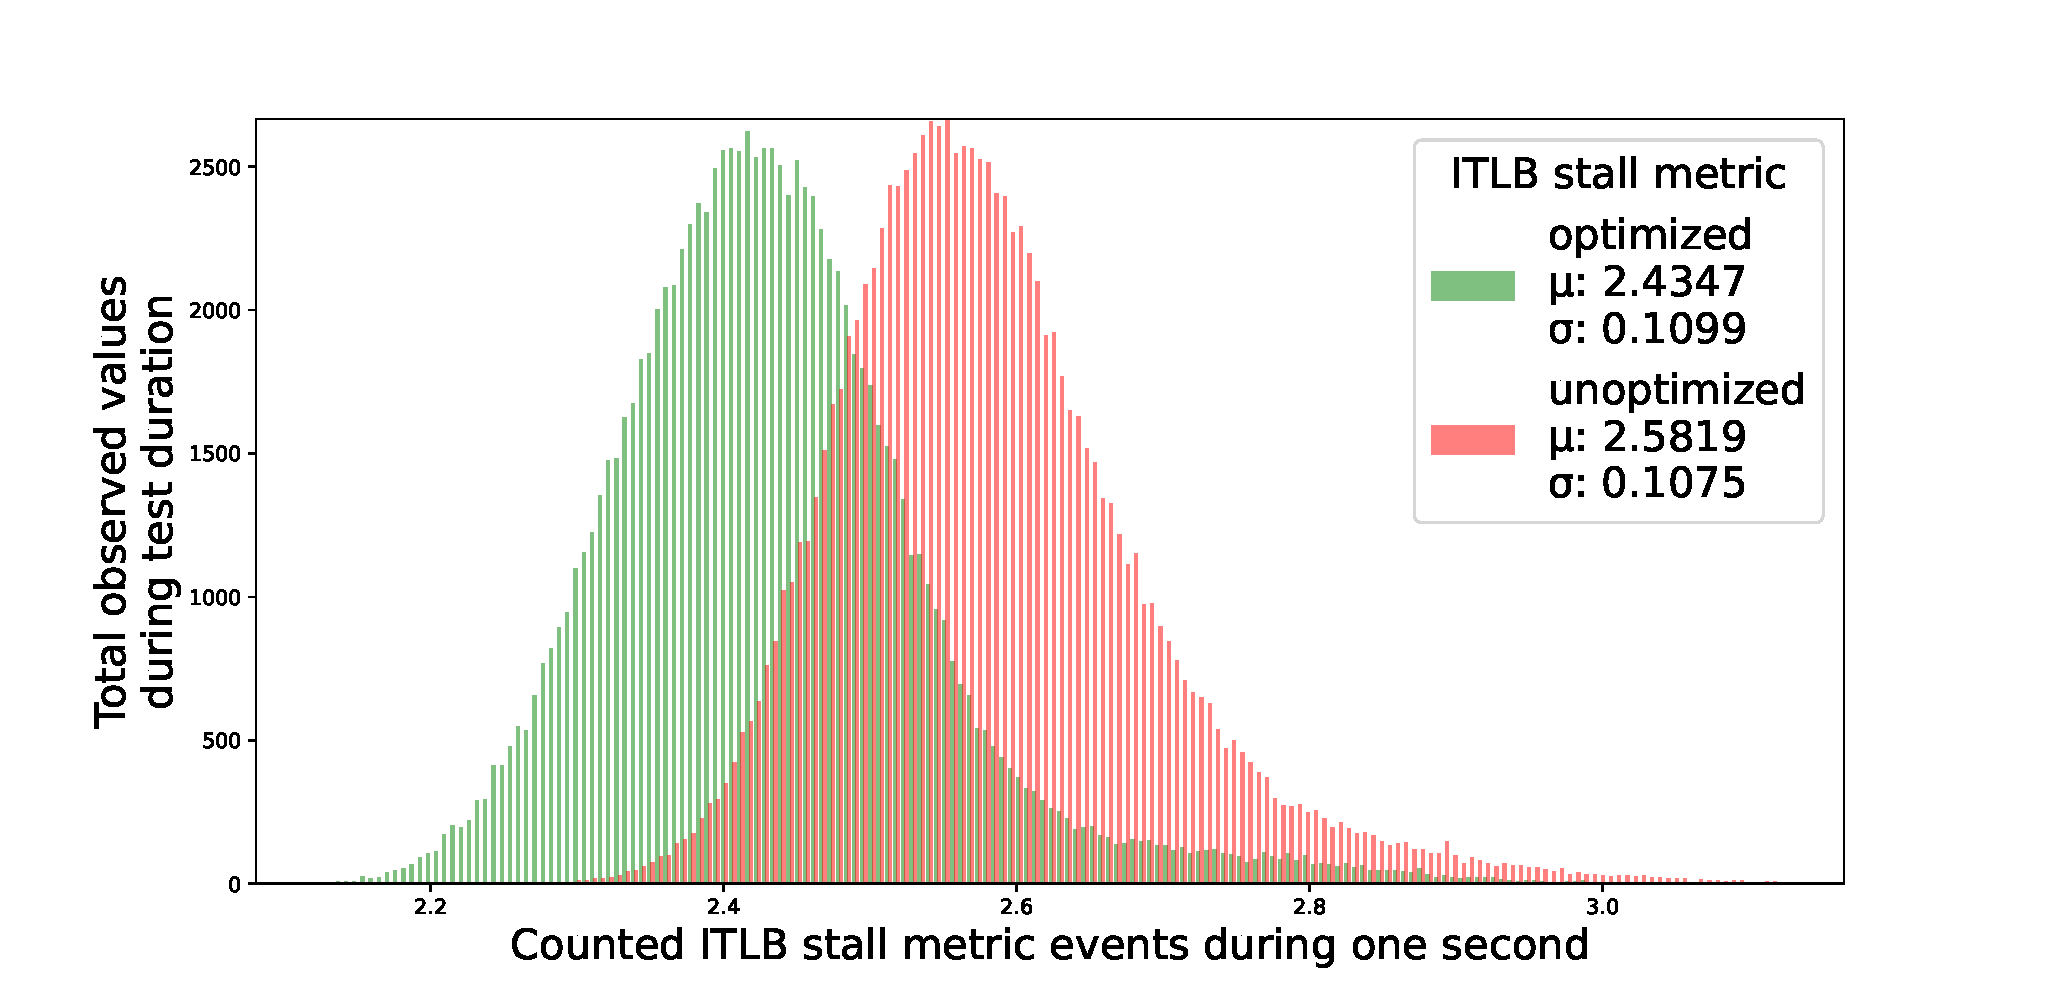
\includegraphics[width=.8\textwidth]{images/5_implementation/itlb-stall.pdf}
        \vspace{.5\baselineskip}
    \end{subfigure}
    \begin{subfigure}{\linewidth}
        \centering
        \captionsetup{singlelinecheck=false, margin={29mm,0cm}}
        \caption{Event frontend\_retired.itlb\_miss}
        \label{fig:histograms-frontend}
        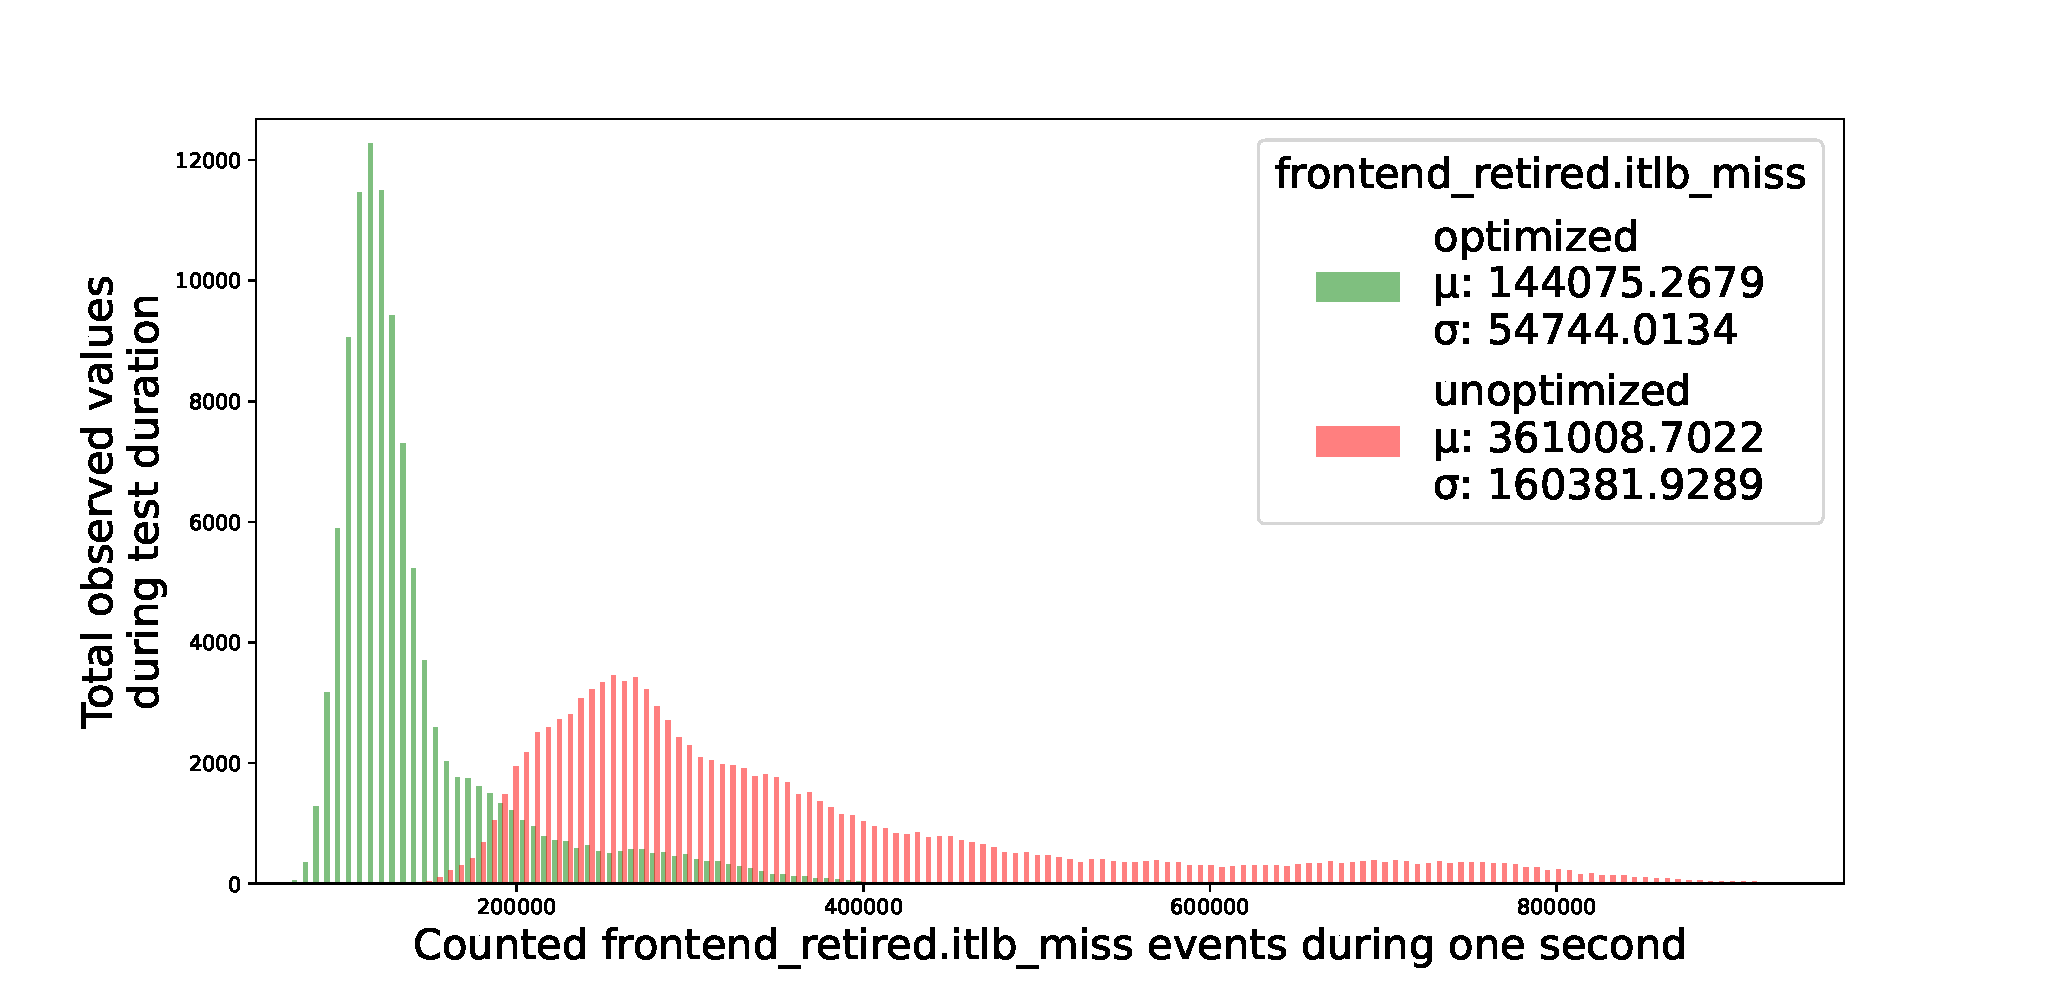
\includegraphics[width=.8\textwidth]{images/5_implementation/frontend-miss.pdf}
    \end{subfigure}
    \caption{Histograms for specific PMU events and metrics for the optimized case (green) and unoptimized case (red)}
    \label{fig:histograms}
\end{figure}
\newpage

Nevertheless, the overall decrease in all events and metrics, particularly in icache\_64b.iftag\_miss, frontend\_retired.itlb\_miss, and the ITLB stall metric, is likely the primary factor behind the observed improvements in the measured network metrics outlined in table \ref{table:throughput}, resulting in an approximate improvement of 14\% for the throughput as well as the total bytes transferred. This is also reflected by an increased IPC value of roughly 0.9\%, as illustrated in table \ref{table:numberresults}.

\chapter{Potential improvements}\label{chapt:improv}

The interpretations presented in chapter \ref{chapt:results} should be taken with a grain of salt as the analysis was conducted on a single Debian release, tested on a single kernel version, for a specific processor model, and with a single workload. Therefore, it is important to consider that the results may not reflect a universal improvement across different combinations of releases, versions, processor models, and workloads.

To provide a more comprehensive and general statement on whether code collocation effectively reduces ITLB pressure in the kernel, it would be necessary to conduct testing and evaluation across a wider range of scenarios. This would involve implementing a more minimal test setup specifically designed to mitigate additional sources of interference, such as minimizing the impact of other applications during the test run.

Moreover, more sophisticated statistical tools should be used to determine if code collocation is statistically significant. For this purpose, non-normal significance tests can be used. \cite[p. 22-25]{patmc} Additionally, it could be beneficial to explore other functionalities that could potentially improve the data collection stages. For example, investigating if the use of the \textit{PEBS} functionality generates more precise stack calls.

\enlargethispage{\baselineskip}
Another area for improvement is the time-consuming process of creating a linker script for every test run and the subsequent recompilation. One way to overcome this could be to hijacking the \textit{Fine-Grained Kernel Address Space Layout Randomization} (FGKASLR) patch \cite{fgkaslrpatch}. Instead of randomizing the kernel code using the Fisher-Yates algorithm, the FGKASLR functionality could be modified to accept a sorted list, enabling the rearrangement of the kernel code based on that list. The FGKASLR patch extends \textit{Kernel Address Space Layout Randomization} (KASLR) by providing a more sophisticated randomised memory layout by rearranging kernel code on a per-function level granularity at load time. \cite{lwnrandom} \cite{fgkaslrartical} This modification could potentially streamline the process and reduce the time required for recompilation.
\chapter{Summary}\label{chapt:summary}

It was shown that code collocation, in conjunction with the C3 heuristic, can effectively reduce ITLB pressure for a specific workload. However, it is important to note that the findings and recommendations presented here are based on a specific Debian release, kernel version, processor model, and workload. For a more general recommendation on whether code collocation effectively reduces ITLB pressure in the kernel, it is highly recommended to conduct further test runs with diverse configurations.

Moreover, it should be noted that code collocation with the C3 heuristic is just one among several techniques that can potentially reduce ITLB pressure. As described in chapter \ref{chapt:heuristic},  the combination of function-sorting with other techniques, which are part of profile guided optimisation, can further contribute to the reduction of ITLB pressure. A project that tries to do this is for example BOLT \cite{llvm-bolt}.

Additionally, there are alternative techniques available, both with and without the use of PGO, that can effectively reduce ITLB pressure. An Intel white paper \cite{intel_opt_runtime} highlights other possibilities, such as leveraging large pages through the use of the \textit{libhugetlbfs} library. The results in \cite{hfsort} indicate that combining the C3 heuristic with huge pages can lead to an even greater reduction of ITLB pressure.
\chapter*{Appendix}\label{appendix:implement}
\addcontentsline{toc}{chapter}{Appendix}

This appendix provides a more detailed description of the commands used in this thesis. Non-essential information has been removed and/or replaced with a simpler version for readability. The complete implementation can be found at \cite{github}.

\section{Call graph creation}\label{appendix:callgraph}

The code snippet in listing \ref{lst:collectdata} provides a unified testing procedure for creating a weighted call graph using \textit{perf}. It initiates the network workload with a defined warm-up time of 10 minutes, then samples the actual number of caller-callee calls in the defined duration. Afterwards, any unused page caches are dropped.

\vspace{.5\baselineskip}
\begin{lstlisting}[
    label={lst:collectdata},
    caption={Commands for executing a call graph collection run}
]
#!/usr/bin/env bash
TIME=140
WARMUP_TIME=$(( 60 * 10 ))

# start workload
workload/network.sh --time $(( TIME + WARMUP_TIME )) \
                    --num-server 20 --dma-buffer 0 &

echo "Wait ${WARMUP_TIME} seconds to warmup..."
sleep $WARMUP_TIME

echo "Start data collection..."
graphrecord.sh --time $TIME \
    --out "$PWD/callgraph-$(date -Iseconds)" \
    --freq 3000`\newpage`
clear_cache(){
    sync; sudo sh -c 'echo 1 > /proc/sys/vm/drop_caches'
}
clear_cache
\end{lstlisting}

More detailed commands on how caller-callee calls are sampled and transformed into a usable form in the \textit{graphrecord.sh} script can be seen in listing \ref{lst:perfrecord}.

\vspace{.5\baselineskip}
\begin{lstlisting}[
    label={lst:perfrecord},
    caption={Simplified commands for generating call graph information with perf}
]
perf record --all-cpus --event cycles:k --branch-filter any,k \
    --freq 3000 --call-graph dwarf,8192 \
    -- sleep ${TIME}

perf report --header --show-info --show-nr-samples --branch-stack \
    --sort sample \
    --fields +symbol_from,symbol_to,symbol_size \
    --percent-limit 0 --field-separator '$' \
    --stdio > "${OUT_FILE}.report"
\end{lstlisting}

\vspace{-\baselineskip}
\section{Network workload}\label{appendix:workload}

A simplified implementation of the network workload can be seen in listing \ref{lst:workload}. It creates multiple instances of client-server pairs that exchange data locally using the zero-copy functionality within a specified time frame. This process occurs in both directions, from client to server and from server to client. Optionally, the script can wait for the applications to complete.

\vspace{.5\baselineskip}
\enlargethispage{2\baselineskip}
\begin{lstlisting}[
    label={lst:workload},
    caption={Commands for running a network workload}
    ]
#!/usr/bin/env bash
IPERF_SERVER_PARAM="--server --daemon --one-off --bind $IP"
IPERF_CLIENT_PARAM="--client $IP --zerocopy --time $TIME"
NICE="sudo nice -n -5" # set nice value for all instances

# start servers
for i in $(seq 1 $NUM_SERVER); do
    S_PORT=$(( 6000 + i ))
    R_PORT=$(( 6000 + NUM_SERVER + i ))

	$NICE iperf3 $IPERF_SERVER_PARAM --port $S_PORT >/dev/null
	$NICE iperf3 $IPERF_SERVER_PARAM --port $R_PORT >/dev/null
done`\newpage`
# start clients
for i in $(seq 1 $NUM_SERVER); do
    TX_PORT=$(( 6000 + i ))
    RX_PORT=$(( 6000 + NUM_SERVER + i ))
    
    $NICE iperf3 $IPERF_CLIENT_PARAM --port $TX_PORT >/dev/null &
    $NICE iperf3 $IPERF_CLIENT_PARAM --port $RX_PORT \
                                     --reverse >/dev/null &
done

# if wait flag is specified wait for all programs to finish
(( WAIT )) && wait -n
\end{lstlisting}

\section{PMU events collection}\label{appendix:events}

Listing \ref{lst:collectsta} provides a unified testing procedure for collecting PMU events. Multiple test runs are executed in a single test. For each test run, it initializes a network workload with a defined warm-up time of 10 minutes, followed by the actual collection of PMU events. Afterwards, it drops any unused page cache for the next test run.

\vspace{.5\baselineskip}
\begin{lstlisting}[
    label={lst:collectsta},
    caption={Commands for starting a PMU events collection run}
]
#!/usr/bin/env bash
TIME=$(( 3600 * 6 ))
WARMUP_TIME=$(( 60 * 10 ))
LOOPS=5

for i in $(seq 1 $LOOPS); do
    # start workload
    workload/network.sh --time $(( TIME + WARMUP_TIME )) \
                        --num-server 20 --dma-buffer 2024 &
    
    echo "Wait ${WARMUP_TIME} seconds to warmup..."
    sleep $WARMUP_TIME
    
    echo "Start PMU events collection..."
    itlbstat.sh --out "$PWD/$i-itlbstats-$(date -Iseconds)" $TIME`\newpage`
    clear_cache(){
        sync; sudo sh -c 'echo 1 > /proc/sys/vm/drop_caches'
    }
    clear_cache
done
\end{lstlisting}

For a more detailed understanding of how the PMU events are sampled and transformed into a usable form in the \textit{itlbstat.sh} script, one can refer to listing \ref{lst:stats}. The defined PMU events and metrices in chapter \ref{section:events} are used for the implementation. In this listing, repetitive or uninteresting code sections have been abbreviated with \textit{[...]}. This implementation is based on the work of Brendan Gregg's script \textit{tlbstat} \cite{tlbstat}.

\vspace{.5\baselineskip}
\begin{lstlisting}[
    label={lst:stats},
    caption={Simplified commands for collecting PMU events},
    commentstyle=\color{black},
    keywordstyle=\color{black},
]
perf stat -e cycles \
    -e itlb_misses.miss_causes_a_walk \
    # [...]
    -e instructions \
    -I $(( 1 * 1000 )) \
    --all-cpus -- sleep ${TIME} 2>&1 | awk \
    -v hlines=0 -v out="${file}.report" -v interval=1 '
    # [...]
    # counters:
    $3 == "cycles" { cycles = $2; }
    $3 == "itlb_misses.miss_causes_a_walk" { imwalk = $2 }
    # [...]
    $3 == "instructions" {
        ins = $2
        # [...]
        out = sprintf("%-10d %-10d # [...] %-10d",
            cycles / 1000,
            imwalk,
            # [...]
            ins / 1000)
        print out
        # [...]
'
\end{lstlisting}

\newpage

\section{Bandwidth test}\label{appendix:bandwidth}

Listing \ref{lst:collectband} describes a unified testing procedure for testing the bandwidth. Multiple test runs are executed in a single test. For each test run, it initializes a network workload with a defined warm-up time of 10 minutes, followed by the actual 1-hour long bandwidth test. Afterwards, any unused page cache is dropped for the next test run.

\vspace{.5\baselineskip}
\begin{lstlisting}[
    label={lst:collectband},
    caption={Commands for starting a bandwidth test}
]
#!/usr/bin/env bash
TIME=$(( 3600 * 1 ))
WARMUP_TIME=$(( 60 * 10 ))
LOOPS=5

COMMON="workload/network.sh --bandwidth --dma-buffer 2024 --wait"

for i in $(seq 1 $LOOPS); do
    OUTPUT="$i-bandwidth.perf"
    
    echo "Wait ${WARMUP_TIME} seconds to warmup..."
    $COMMON --time $WARMUP_TIME --out $OUTPUT
    
    echo "Start bandwidth test..."
    $COMMON --time $TIME --out $OUTPUT
    
    clear_cache(){
        sync; sudo sh -c 'echo 1 > /proc/sys/vm/drop_caches'
    }
    clear_cache
done
\end{lstlisting}

\vspace{-\baselineskip}

A simplified implementation of the bandwidth test, which is called via \textit{workload/network.sh --bandwidth}, can be seen in listing \ref{lst:bandwidth}. It creates a single client-server instance and captures the output of the client. It exchanges data locally using the zero-copy functionality within a specified time frame.

\enlargethispage{2\baselineskip}
\vspace{.5\baselineskip}
\begin{lstlisting}[
    label={lst:bandwidth},
    caption={Simplified commands for executing a bandwidth test}
]
#!/usr/bin/env bash
B_SERVER_PARAM="--server --daemon --one-off --bind $IP"
B_CLIENT_PARAM="--client $IP --zerocopy --time $TIME --format k"
NICE="sudo nice -n -5" # set nice value for all instances

$NICE iperf3 $B_SERVER_PARAM --port 6000 >/dev/null
$NICE iperf3 $B_CLIENT_PARAM --port 6000 > "$OUTPUT"
\end{lstlisting}

\sloppy % set sloppy tolerances
\printbibliography[heading=bibintoc]
%\printbibliography[keyword=pic, title={Pictures only}]
\end{document}
